\chapter{Einführung in Deep Learning}

    \begin{figure}[h]
        \centering
        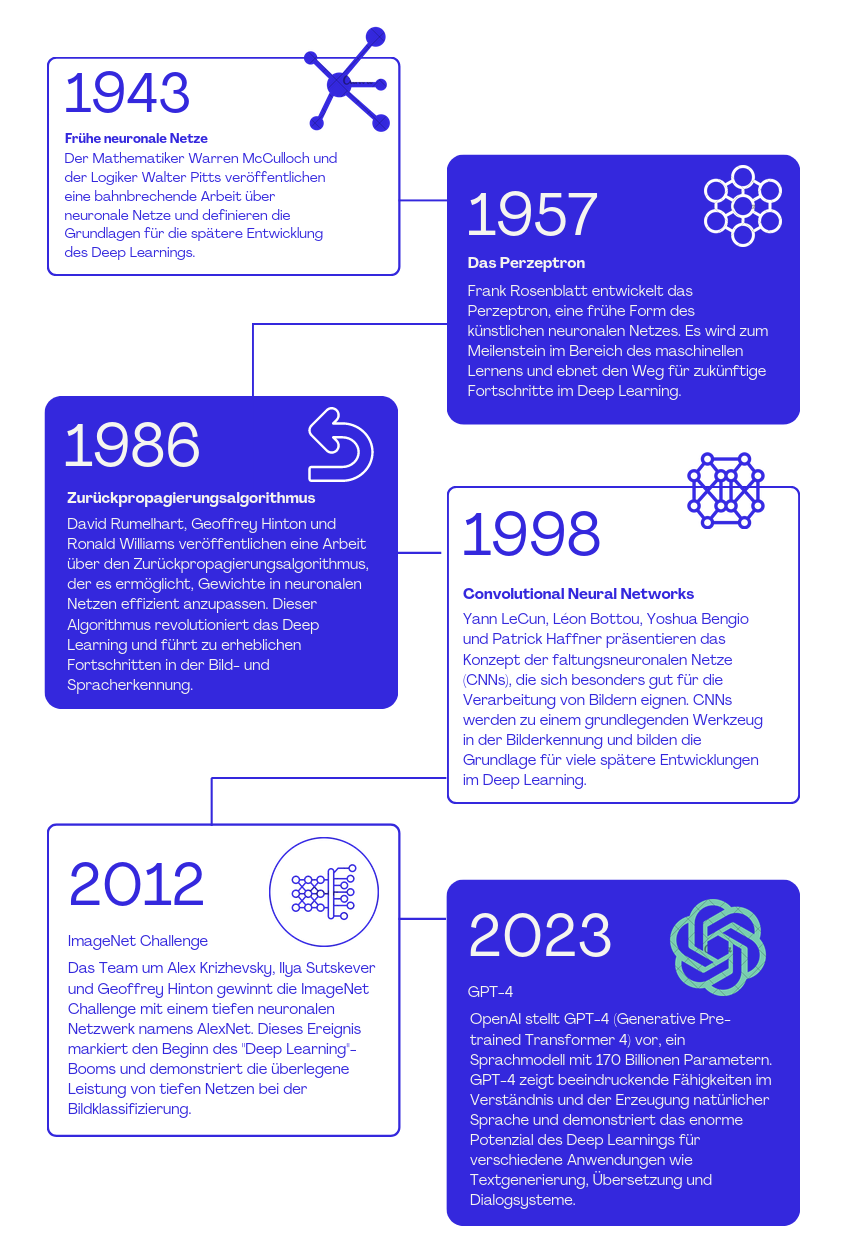
\includegraphics[width=\textwidth]{img/timeline.png}
        \caption{Timeline der Geschichte von Deep Learning}
        \label{fig:deeplearning_timeline}
    \end{figure}

    Deep Learning ist eine Unterkategorie des maschinellen Lernens und beschäftigt sich mit der Entwicklung und Anwendung von neuronalen Netzwerken mit mehreren Schichten, um komplexe Probleme zu lösen. Es verwendet künstliche Intelligenz, um aus großen Datenmengen Muster zu erkennen und Entscheidungen zu treffen. 
    In der heutigen Welt hat Deep Learning Anwendungen in Bereichen wie Spracherkennung, Bilderkennung, Robotik, Medizin und Autonomen Fahrzeugen gefunden. 
    Die Geschichte des Deep Learning reicht zurück bis in die 1940er Jahre, aber erst in den 2000er Jahren wurden die Algorithmen und Computerleistung ausreichend entwickelt, um Deep Learning erfolgreich anzuwenden. 
    Im Jahr 2012 gewann ein Deep Learning-Modell namens AlexNet den ImageNet-Wettbewerb, was als Durchbruch für die Anwendung von Deep Learning in Computer Vision gilt.
    Traditionelles maschinelles Lernen verwendet in der Regel flache neuronale Netzwerke, die nur eine Schicht haben, um Daten zu analysieren. 
    Im Gegensatz dazu verwenden Deep-Learning-Modelle mehrere Schichten, um komplexere Merkmale der Daten zu identifizieren. 
    Dies ermöglicht eine höhere Genauigkeit und Effektivität bei der Lösung komplexer Probleme.
    Beispiele für reale Anwendungen von Deep Learning sind unter anderem die Bilderkennung in sozialen Medien, die Spracherkennung in Smart Speakern wie Amazon Echo und Google Home, sowie die automatisierte Diagnose von medizinischen Bildern wie CT-Scans und MRT-Bildern.

\section{Motivation der Studie von CNNs und deren Training}
    
    Traditionelle maschinelle Lernalgorithmen sind nicht effektiv bei der Verarbeitung komplexer Datentypen wie Bildern. Hier kommen Convolutional Neural Networks (CNNs) ins Spiel. 
    CNNs sind eine spezielle Art von neuronalem Netzwerk, die speziell für die Bilderkennung und Computer Vision entwickelt wurden. 
    CNNs arbeiten durch die Verwendung von Filtern, die über das Eingabebild geschoben werden, um Merkmale wie Kanten, Farben und Texturen zu extrahieren. 
    Diese Merkmale werden dann von Schichten von Neuronen verwendet, um die Merkmale zu kombinieren und eine Vorhersage zu treffen. 
    Eine der größten Herausforderungen beim Training von CNNs ist das Overfitting, bei dem das Modell zu stark auf die Trainingsdaten optimiert wird und dadurch bei neuen Daten schlecht abschneidet. 
    Eine weitere Herausforderung ist das Problem der verschwindenden Gradienten, bei dem die Gradienten, die zur Anpassung der Gewichte verwendet werden, während des Trainings immer kleiner werden und das Modell nicht mehr lernen kann. 
    Um diese Probleme zu lösen, werden Optimierungsalgorithmen wie der stochastische Gradientenabstieg verwendet, um die Gewichte des Modells anzupassen und das Modell an die Daten anzupassen. 
    Es gibt auch Techniken wie Dropout und Data Augmentation, die dazu beitragen können, Overfitting zu reduzieren. 
    Es ist wichtig, CNNs zu verstehen und effektiv zu trainieren, um die volle Leistungsfähigkeit von Deep Learning in der Bilderkennung und Computer Vision zu nutzen. 
    
\section{Struktur der Arbeit}

    Diese Studienarbeit ist in drei Hauptabschnitte unterteilt.
    Im ersten Abschnitt wird eine Einführung in Deep Learning gegeben, einschließlich der Bedeutung von Deep Learning in der heutigen Welt, der Geschichte und Entwicklung des Deep Learning, der Unterschiede zwischen Deep Learning und traditionellem maschinellem Lernen und Beispielen für reale Anwendungen von Deep Learning.
    
    Im zweiten Abschnitt wird die Motivation hinter der Studie von CNNs und deren Training erläutert. Dabei werden die Einschränkungen von traditionellen maschinellen Lernalgorithmen bei der Verarbeitung komplexer Datentypen wie Bildern diskutiert und die Bedeutung von CNNs bei der Bilderkennung und Computer Vision erklärt. Weiterhin werden die Herausforderungen beim Training von CNNs wie Overfitting und verschwindende Gradienten sowie die Rolle von Optimierungsalgorithmen wie dem stochastischen Gradientenabstieg beim Training von CNNs beschrieben.
    
    Im dritten Abschnitt werden die Ergebnisse und Beiträge dieses Papiers skizziert. Dies beinhaltet eine Zusammenfassung der wichtigsten Erkenntnisse und Empfehlungen für das effektive Training von CNNs.